\documentclass[12pt,letterpaper,titlepage]{article}

\usepackage{fontspec}
\defaultfontfeatures{Mapping=tex-text}
\usepackage{xunicode}
\usepackage{xltxtra}
\usepackage{amsmath}
\usepackage{pdfpages}
\usepackage{amsfonts}
\usepackage{bbold}
\usepackage{amssymb}
\setcounter{secnumdepth}{0}
\usepackage{nameref}
\usepackage{enumitem}
\usepackage{environ}
\usepackage{pgfplots}
\usepackage{listings}

\showboxdepth=\maxdimen
\showboxbreadth=\maxdimen


\usepackage{paracol}
\usepackage{wrapfig}
\globalcounter{table}
\globalcounter{figure}
\usepackage{graphicx}
\usepackage[left=1in,right=1in,top=1in,bottom=1in]{geometry}
\graphicspath{{img/}}

\author{Jacob Abel}
\title{	Design \& Simulate 25
	\\\large ECE2204 CRN:82929
}

\setlength{\parskip}{0.5em}

\begin{document}
\maketitle
\begin{raggedright}
\columnratio{0.59}
\begin{paracol}{2}
\switchcolumn
\begin{center}
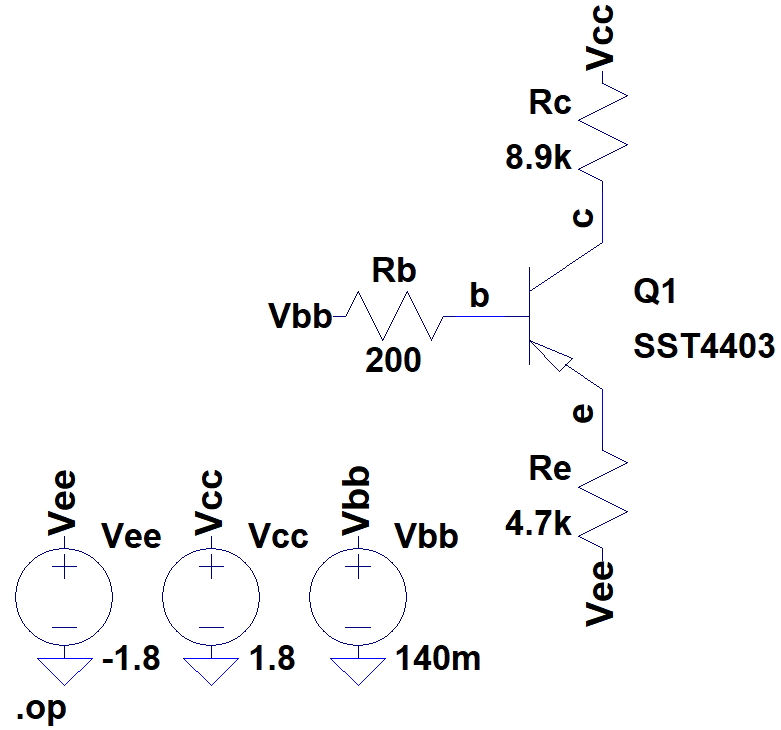
\includegraphics[width=\textwidth, height=12\baselineskip, keepaspectratio=true]{ds2}
\end{center}
\switchcolumn

\section{Problem 25.5-7.b.1: } 
\subsection{Design}
Calculate the power of the transistor. The transistor is currently in Saturation mode with $\beta = 150$, $V_{ECon} = 0.465V$, and $V_{EBon} = 0.615V$.

\end{paracol}
\clearpage
\subsection{Validation}

\begin{center}
LTSpice Implementation (All values of truth table match waveform)
\columnratio{0.5}
\begin{paracol}{2}
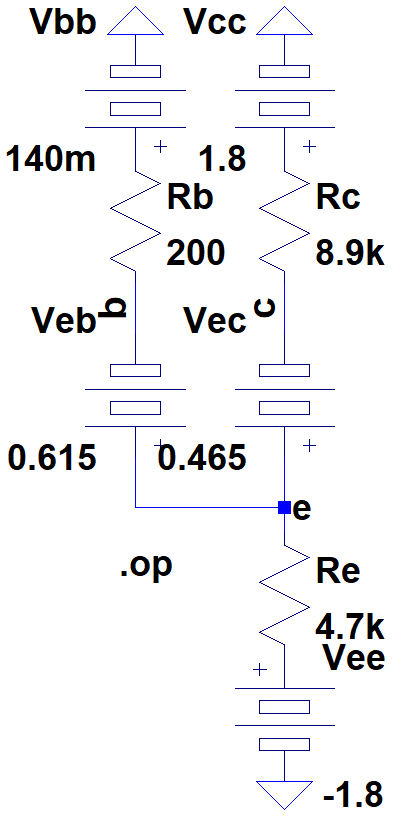
\includegraphics[width=\textwidth, height=25\baselineskip, keepaspectratio=true]{ds2b}
\switchcolumn
\begin{tabular}{|r|l|c|}
  \hline V(e):	  & 0.683066	 & voltage
\\\hline V(b):	  & 0.0700664	 & voltage
\\\hline V(c):	  & 0.210066	 & voltage
\\\hline V(p001): & 0.14	     & voltage
\\\hline V(p002): & 1.8	         & voltage
\\\hline V(p003): & -1.8	     & voltage
\\\hline I(Re):	  & 0.000528312  & device\_current
\\\hline I(Rc):	  & 0.000178644  & device\_current
\\\hline I(Rb):	  & 0.000349668  & device\_current
\\\hline I(Vee):  & 0.000528312  & device\_current
\\\hline I(Vcc):  & -0.000178644 & device\_current
\\\hline I(Vbb):  & -0.000349668 & device\_current
\\\hline I(Vec):  & -0.000178644 & device\_current
\\\hline I(Veb):  & -0.000349668 & device\_current
\\\hline
\end{tabular}
\end{paracol}
\end{center}

This problem should demonstrate a basic ability to analyse basic BJT circuits. 

\textit{I have neither given nor received unauthorized assistance on this assignment.}


\end{raggedright}
\end{document}
